\documentclass[11pt,a4paper]{article}
\usepackage[margin=25mm]{geometry}
\usepackage{amsmath,amssymb,graphicx,booktabs,tabularx,array,xcolor}
\usepackage[colorlinks=true,urlcolor=teal,citecolor=teal,linkcolor=teal]{hyperref}
\usepackage{fancyhdr}
\pagestyle{fancy}\fancyhf{}\lhead{Binaural Hearing Lab}\rhead{Research edition 0.2}\cfoot{\thepage}
\setlength{\headheight}{14pt}\setlength{\parindent}{0pt}\setlength{\parskip}{4pt}
\newcolumntype{Y}{>{\raggedright\arraybackslash}X}
\newcommand{\code}[1]{\texttt{#1}}
\title{\Huge Binaural Hearing Lab\\[8mm]\Large From hearing impairment to reproducible hearing-aid signal processing}
\author{Research implementation prepared for Aditya Raikar\\Implementation and documentation: Codex}
\date{25 November 2026}
\begin{document}
\maketitle
\begin{abstract}
This white paper specifies a research and teaching platform for connecting auditory impairment, signal-processing choices and experimental evidence. The first implementation combines measured binaural acoustics, audiogram-conditioned gain targets, an educational compressor, interactive listening controls and a separate hearing-model experiment. A curated literature map spans classical multichannel filtering, neural enhancement and emerging low-latency binaural methods. The central design rule is traceability: distinguish published findings, local measurements, pedagogic approximations and unimplemented candidates. The initial HASPI experiment is a one-utterance feasibility pilot, not a comparative clinical study. The browser is a streaming demonstration, not a wearable hearing aid or a calibrated diagnostic tool.
\end{abstract}
\vspace{6mm}
\textbf{Delivered artifacts.} Static browser application; source and unit tests; data restoration and provenance; exact offline NAL-R/MSBG/HASPI experiment; compute benchmark; this editable \LaTeX{} document; \code{README.md}, \code{requirements.txt} and \code{Skills.md}.

\textbf{Scope boundary.} Actual microphone-array beamforming, estimated localization, neural enhancement, source separation and feedback cancellation are future modules. Their literature entries do not imply that they currently run in the demo. Normal-hearing headphone listening to an altered signal cannot establish what a particular hearing-impaired person experiences.
\newpage
\section{Research questions and evidence strategy}
The intended lab asks four linked questions: (1) which auditory limitations are being modeled; (2) what information each algorithm has at run time; (3) what the processing changes in audibility, quality and spatial cues; and (4) whether the complete implementation meets device constraints. A visually convincing demo should not obscure these distinctions.

\begin{tabularx}{\linewidth}{@{}p{.22\linewidth}YY@{}}\toprule
Question & Controlled comparison & Evidence needed\\\midrule
Audibility & Unprocessed versus prescribed gain & Level calibration, audiogram, response verification\\
Dynamic range & Fixed gain versus WDRC & Input/output curves, envelope effects, loudness validation\\
Noise and target selection & Monaural, multichannel and neural enhancement & Shared mixtures, target distortion, intelligibility and quality\\
Spatial hearing & Independent-ear versus binaural processing & Target and residual-noise ITD/ILD, localization tests\\
Practical feasibility & Offline versus streaming and hardware & Lookahead, buffers, compute tails, memory, energy and loopback delay\\\bottomrule
\end{tabularx}

This is an initial \emph{scoping survey}, not a systematic review. Searches used primary papers, institutional repositories, official datasets and upstream implementation documentation. Inclusion favored methods with a clear hearing-aid connection, explicit latency discussion, reproducible code or a foundational role. The selection spans older interpretable baselines and current candidates through 25 November 2026. It is not exhaustive; the latest two 2026 entries were screened at abstract level only.

No ranking combines results from unrelated datasets. An improvement reported in a paper remains a published claim until this repository reproduces it. A model that works faster than real time on a workstation is not thereby suitable for an open-fit hearing aid. Likewise, auditory-model scores remain predictions rather than measured listener benefit.

\textbf{Reproduction status.} The live browser runs an approximate NAL-R-target filter bank, WDRC and an oracle directional illustration. The offline pilot calls the established Clarity implementations of NAL-R, MSBG and HASPI. It evaluates a different, exact FIR realization of NAL-R, not the browser approximation. Neural candidates are not loaded or timed by this version.
\section{Why hearing loss happens}
Sound reaches the eardrum through the outer ear; middle-ear motion couples energy into the cochlea. Hair-cell transduction and neural signaling carry information to the brain. Noise, aging, disease and some medicines can damage this pathway; the location and mechanism of damage matter for compensation. Hearing aids increase access to sound through the remaining auditory system rather than restoring damaged sensory structures \cite{nidcd}.

Conductive loss involves impaired transmission through the outer or middle ear. Sensorineural loss involves cochlear or neural dysfunction. Mixed loss combines components. This lab focuses on a simplified cochlear-loss teaching scenario; it does not diagnose the type or cause from an audiogram.
\newpage
\section{Auditory deficits and what technology can compensate}
Outer-hair-cell dysfunction can reduce low-level sensitivity, cochlear compression and frequency selectivity. Inner-hair-cell, synaptic or neural dysfunction can further restrict the information available to the listener. These mechanisms may coexist, and their contributions are not uniquely recoverable from pure-tone thresholds. Loudness models distinguish threshold elevation from the loss of compressive behavior and broadened excitation patterns \cite{moore2014}.

An audiogram reports threshold in dB HL at test frequencies. dB HL is referenced to normal thresholds under standardized measurement conditions, not equal to dB SPL and not a number to subtract directly from a digital waveform for a physiological simulation. Two listeners with similar audiograms may have different suprathreshold abilities and listening needs.

\begin{tabularx}{\linewidth}{@{}p{.23\linewidth}YY@{}}\toprule
Deficit or problem & Technology response & Remaining limitation\\\midrule
Reduced audibility & Frequency-dependent gain & Gain does not recover missing sensory coding\\
Reduced dynamic range / recruitment & Wide dynamic-range compression & Time constants may alter envelopes and spatial cues\\
Reduced selectivity & Better input SNR via directional or neural processing & Filtering cannot restore normal cochlear tuning\\
Competing speech & Target selection, spatial filtering or separation & Wrong-target capture and artifacts can be harmful\\
Spatial-cue disruption & Joint binaural constraints and linked control & Noise suppression competes with environmental awareness\\
Feedback instability & Adaptive feedback control, gain limits, physical fitting & Desired/output correlation and changing paths complicate adaptation\\\bottomrule
\end{tabularx}

\subsection{Why amplification is not a simple inverse of loss}
A fixed gain cannot simultaneously make soft speech audible and keep intense sound comfortable when the usable dynamic range has narrowed. WDRC therefore gives more gain to lower-level inputs than to higher-level inputs. Its behavior depends on channel bandwidth, level detector, attack/release constants and inter-channel interaction \cite{kates2005}. These engineering choices cannot be inferred solely from an audiogram.

The live B/C modes apply bandwise attenuation numerically shaped by the audiogram. This is explicitly an \emph{audibility illustration}. It omits realistic recruitment, auditory-filter broadening, temporal coding and individual neural factors. A separate offline MSBG example gives a more developed model-based auralization \cite{clarity,moore1997}; even that model cannot be treated as the literal experience of an individual.

\subsection{Which frequencies should be enhanced?}
There is no universal frequency band that maximizes useful hearing. Gain should depend on the listener's thresholds, input level, residual dynamic range, speech information and output constraints. High-frequency consonant information can matter, but indiscriminate high-frequency boost can increase noise, distortion or discomfort. Some losses limit the usefulness of extra gain. A good objective score on its own is not a fitting prescription.
\newpage
\section{Conventional and binaural hearing-aid processing}
A representative processing chain contains microphone acquisition, feedback management, directional or multichannel enhancement, gain/compression, output limiting and receiver playback. Implementations may reorder or jointly optimize stages. Their interactions matter: a denoiser changes the level estimate driving compression; compression can bring up residual noise; independent left/right gain control can change interaural level differences.

With microphone signals $x_m(t)$ and source signals $s_q(t)$, a scene model is
\begin{equation}
 x_m(t)=\sum_q h_{mq}(t)*s_q(t)+v_m(t),
\end{equation}
where $h_{mq}$ must correspond to the actual microphone position. An ear-canal HRIR is not interchangeable with a behind-the-ear microphone response. A system using multiple microphones per side needs the associated transfer functions or recordings.

\subsection{Beamforming, localization and separation}
A frequency-domain beamformer produces $y=\mathbf{w}^{H}\mathbf{x}$. For a narrowband target steering vector $\mathbf{d}$ and noise covariance $\mathbf{R}_{nn}$, the ideal MVDR solution is
\begin{equation}
\mathbf{w}_{\mathrm{MVDR}}=\frac{\mathbf{R}_{nn}^{-1}\mathbf{d}}{\mathbf{d}^{H}\mathbf{R}_{nn}^{-1}\mathbf{d}}.
\end{equation}
Practical estimation errors, diagonal loading, target motion and adaptation time must be specified. Knowing the simulated target direction is oracle information; estimating it from mixture microphones is a different experiment. Source separation additionally requires a target-selection convention so that a cleaner output of the wrong speaker is not scored as success.

Binaural MWF and MWF-N provide a foundational comparison between noise reduction and spatial preservation \cite{mwf}. Their relevance is that both desired speech and residual noise convey spatial information. Suppressing all noise as strongly as possible is not equivalent to maintaining useful environmental awareness. The current demo's directional toggle simply changes separate target/noise stem gains; it is not an implementation of these filters.

\subsection{HRTFs: simulation versus a physical device}
This lab uses HRTFs through their time-domain HRIRs to produce ear signals from virtual source locations. In physical use the head, torso and pinna already filter acoustic sound before it reaches the device. A hearing aid does not generally add a second generic HRTF to make that sound binaural. HRTFs and device-specific transfer functions are nevertheless useful for simulation, steering, training and spatial-cue analysis \cite{kemar}.

Generic head data also limits the headphone illusion: individualized geometry and headphone equalization affect localization. Head motion and room reflections are further variables. Our scene includes only horizontal anechoic directions, not a reverberant room or measured head tracking.
\newpage
\section{Echo, feedback and delay}
In an acoustic feedback loop, the receiver output leaks into the input microphones. A simplified model is $x(t)=s(t)+f(t)*y(t)$, with amplification/enhancement producing $y$. Loop gain and phase can lead to instability. An adaptive canceller estimates $f$ from a receiver reference and subtracts its predicted contribution, but the desired signal and receiver output are correlated. Delay, decorrelation, adaptation control and path-change robustness must therefore be considered.

Automotive or teleconference acoustic echo cancellation usually removes a known far-end loudspeaker signal from a microphone capture path. Hearing-aid feedback cancellation addresses a local closed loop whose output originates from the desired input. The adaptive-filter mathematics overlaps, while the identification conditions and performance criteria differ. This version implements neither AEC nor a feedback canceller. A proposed extension will evaluate an explicit loop using maximum stable gain, misalignment and speech distortion, including changing feedback paths.

\subsection{Direct-path interference}
An open fitting can mix a nearly direct acoustic path with a delayed processed path. For a simple scalar-gain example,
\begin{equation}
 z(t)=\alpha x(t)+(1-\alpha)g\,x(t-\tau),
\end{equation}
whose frequency response can exhibit comb filtering. The browser's D mode includes this illustrative mixture with user-controlled added delay and direct fraction. It is not an acoustic-feedback simulation and its delay slider does not include browser or hardware latency.

\subsection{Three quantities that must not be conflated}
\begin{enumerate}
\item \textbf{Algorithmic delay}: lookahead, reconstruction and frequency-dependent filter/group delay, under an explicitly stated convention.
\item \textbf{Compute cost}: processing time, operation count, RAM and energy. Average processing faster than incoming audio does not bound worst-case deadline failures.
\item \textbf{End-to-end delay}: microphone and ADC, buffers, processing scheduling, transport, DAC and receiver and acoustic paths. Measure it with an appropriate loopback experiment.
\end{enumerate}

A $128$-sample block at $44.1$ kHz spans $2.9025$ ms. That number is a scheduling interval, not the complete latency. Open-fit constraints make the distinction particularly consequential. Low-latency research often changes synthesis design while retaining longer causal analysis context \cite{wu2025,deepfir}.
\section{Open research resources}
MIT KEMAR provides measured head-related data with attribution terms \cite{kemar}. LibriSpeech supplies openly licensed speech \cite{librispeech}. Clarity supplies hearing-aid-oriented scenes, listener profiles, evaluators and baselines \cite{clarity}. These are complementary resources, not interchangeable benchmarks. openMHA is a platform for real-time hearing-aid research rather than a single competing algorithm \cite{openmha}.
\newpage
\section{Literature map: classical to current candidates}
\begin{tabularx}{\linewidth}{@{}p{.24\linewidth}YY@{}}\toprule
Method & Why include it & Current local status\\\midrule
NAL-R \cite{nalr} & Transparent historical gain baseline & Target approximation live; exact FIR offline\\
WDRC \cite{kates2005} & Level-dependent compensation & Educational live implementation\\
MSBG / HASPI \cite{clarity,haspi} & Hearing-aware modeling and evaluation & Offline pilot executed\\
Binaural MWF/MWF-N \cite{mwf} & Cue-preservation tradeoff & Literature candidate\\
DeepFilterNet \cite{dfn} & Open efficient deep-filtering baseline & Not reproduced here\\
Deep FIR / Viking \cite{deepfir} & Samplewise filtering and very short delay & Full paper reviewed; not reproduced\\
Wu--Braun study \cite{wu2025} & Controlled low-latency design comparison & Full paper reviewed; not reproduced\\
RT-Tango \cite{rttango} & Distributed binaural computation & 2026 abstract screened only\\
Directivity-conditioned filtering \cite{uphaus} & Steerable neural spatial filtering & 2026 abstract screened only\\\bottomrule
\end{tabularx}

DeepFilterNet combines perceptually motivated features and complex filtering; its published real-time demonstration reports workstation efficiency and available code/weights \cite{dfn}. This makes it a practical reproduction candidate, but neither low RTF nor independent mono application establishes hearing-aid latency or binaural-cue preservation.

Deep FIR uses a compact recurrent model to predict FIR filters and reduces delay through synthesis design and minimum-phase conversion. The paper reports mean algorithmic latency of $0.32$--$1.25$ ms and mean end-to-end latency of $3.35$ ms on its hardware \cite{deepfir}. Those are published results, not measurements of our implementation. Code and checkpoint readiness must be separately verified before selecting a reproduction configuration.

Wu and Braun compare low-latency techniques within a controlled enhancement study, including asymmetric and learnable windows, adaptive time-domain filter banks and prediction \cite{wu2025}. Their experimental framing motivates our requirement to change one module while retaining shared training/evaluation conditions, instead of comparing headline numbers from unrelated systems.

Two newer candidates expand the survey's scope. RT-Tango's abstract describes distributed binaural processing with ERB compression, grouped recurrent inference and asymmetric STFT, reporting operation as low as $8$ ms \cite{rttango}. Directivity-conditioned filtering reports a $10$ ms design with FiLM steering and a cross-channel relationship loss \cite{uphaus}. These abstract-level entries are candidates, not endorsed reproductions or proof of suitability for every fitting. No local scores are attached to them.

The important research issue is a Pareto tradeoff across audibility, intelligibility, quality, spatial awareness, latency and power. A single score cannot summarize all of these requirements.
\newpage
\section{The implemented browser signal path}
\subsection{Scene renderer and persistent state}
The engine runs at $44{,}100$ Hz and maintains source positions, FIR histories, filter-bank states, envelopes and delay buffers across blocks. Two sources are convolved with separate left/right measured HRIRs:
\begin{equation}
 x_e[n]=\sum_{q=1}^{2}\sum_{k=0}^{127}h_{e,q}[k]s_q[n-k],\qquad e\in\{L,R\}.
\end{equation}
The compact KEMAR set is reduced to 37 horizontal directions at $5^{\circ}$ spacing. Negative azimuth swaps ears. Nearest-direction selection and a 20 ms coefficient transition avoid instantaneous HRIR switching; this is not physically continuous motion interpolation. Original coefficient scale is retained.

Browser speech is normalized to RMS $0.05$ before spatialization. Edge fades reduce looping discontinuities. Synthetic noise uses a seeded uniform sequence followed by a one-pole lowpass; its gain targets the same expected RMS before SNR scaling. Quiet sets the masker to zero. User microphone input is uncalibrated, so the scene SNR label is not a measured microphone SNR.

\subsection{NAL-R target gains}
Let $H_i$ be thresholds at $[250,500,1000,2000,4000,6000]$ Hz and $S=H_{500}+H_{1000}+H_{2000}$. The implemented target follows the Clarity realization of NAL-R \cite{nalr,clarity}:
\begin{align}
 A&=\begin{cases}0.05S,&S\leq180\\9+0.116(S-180),&S>180,\end{cases}\\
 G_i&=\max(0,A+0.31H_i+C_i),\\
 \mathbf C&=[-17,-8,1,-1,-2,-2]\ \mathrm{dB}.
\end{align}
A zero-loss profile is explicitly bypassed. For the illustrated sloping audiogram, targets are $[0,0.65,12.75,15.4,19.05,20.6]$ dB. This historical linear prescription is selected for transparency; it is not NAL-NL2 or a contemporary individualized fitting recommendation.

\subsection{Broadband reconstruction and compression}
Five lowpasses at $354,707,1414,2828,4899$ Hz form six bands by successive differences plus a final residual. Their sum is exactly the input at unity gain. Unequal gain response differs from the six target samples because the bands overlap widely. The figure on the next page exposes that difference rather than claiming exact matching.

A per-band absolute-value envelope $E[n]$ uses attack or release coefficient $a=\exp[-1/(f_s\tau)]$ and $E[n]=aE[n-1]+(1-a)|b[n]|$. For nominal level $L=100+20\log_{10}(E+\epsilon)$, compression correction is
\begin{equation}
 G_{\mathrm{comp}}(L)=\max(0,L-55)(1/R-1).
\end{equation}
Defaults are $R=2$, attack $10$ ms and release $150$ ms. The level mapping is a numerical assumption, not headphone SPL calibration.
\newpage
\begin{center}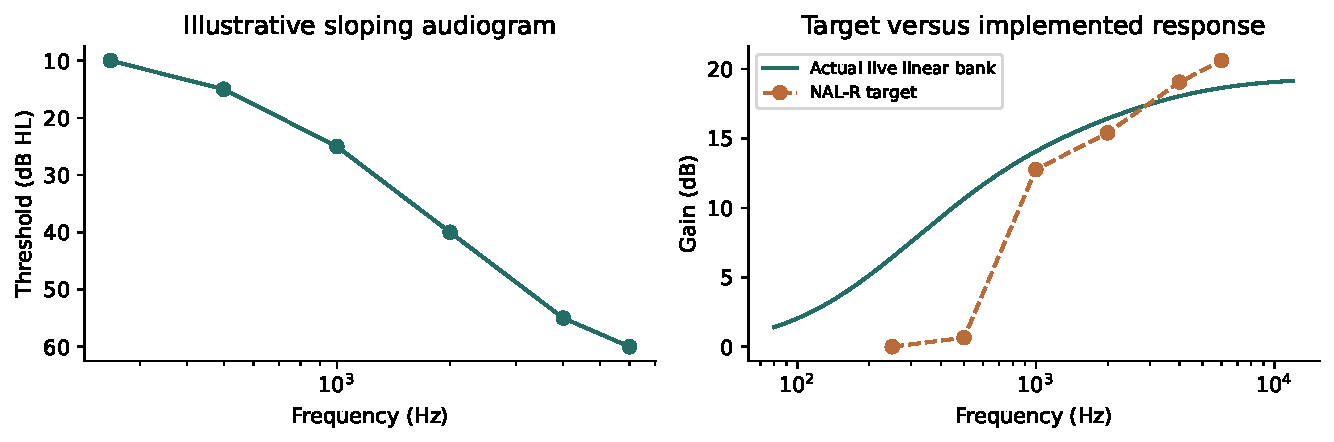
\includegraphics[width=\linewidth]{dist/figures/gain-response.pdf}\end{center}
\textbf{Interpretation.} The right panel shows the steady-state linear filter-bank response with compression disabled. Target dots do not imply that narrow-band gain is realized exactly. This is an implementation limitation to address before clinical or benchmark fitting claims.

\subsection{Four listening conditions}
\begin{tabularx}{\linewidth}{@{}p{.08\linewidth}p{.26\linewidth}Y@{}}\toprule
Mode & Path & Interpretation\\\midrule
A & Spatial reference & Unprocessed virtual ear signals\\
B & Reference + loss attenuation & Educational audibility reduction only\\
C & Gain + WDRC + loss attenuation & Aided illustration through the same simplified attenuation\\
D & Gain + WDRC & Device output before an impaired auditory system\\\bottomrule
\end{tabularx}

Modes B/C use $-H_i$ dB band attenuation as a deliberately simplified illustration. This is not an inverse model of cochlear pathology. In D, direct-path mixing and added delay can be varied. The ideal directional toggle applies $0.15+0.85(1+\cos\theta)/2$ to known source stems before spatialization, and therefore has oracle information. A real beamformer must operate only on mixture microphone signals.

The final master gain defaults to $-24$ dB with smoothing; a hard $\pm0.89$ sample ceiling bounds digital values. The ceiling is not a calibrated hearing-safety limit and may itself introduce distortion. Mode/gain changes are interactive and can produce transients; this prototype does not claim artifact-free clinical switching.

\section{Offline reference experiment}
The executable pilot uses LibriSpeech utterance \code{6930-75918-0000}, resampled to $44.1$ kHz. Its full-clip RMS is set to $65$ dB SPL under a numerical $100$ dB SPL per $0$ dBFS mapping. The illustrated audiogram is $[10,15,25,40,55,60]$ dB HL. Seed $20261125$ controls stationary white noise at $0,5,10,15$ dB SNR plus a quiet condition.

The exact Clarity NAL-R filter has order 220 (221 taps); its 110-sample group delay is removed \emph{offline} for alignment. This does not remove physical device latency. HASPI v2 receives the audiogram and level parameter 100, consistent with the already-scaled reference. Scores are computed on unprocessed or NAL-R outputs, not MSBG-transformed signals. MSBG is rendered separately for listening; cascading another impairment model into HASPI would change the intended evaluation.
\newpage
\textbf{Measured pilot.} Duration 3.505 seconds; pyclarity 0.9.0.\par
\begin{center}\begin{tabular}{lrrr}\toprule
SNR & Unaided HASPI & NAL-R HASPI & Difference\\\midrule
0 dB & 0.7796 & 0.8271 & 0.0474 \\
5 dB & 0.9093 & 0.9419 & 0.0326 \\
10 dB & 0.9568 & 0.9748 & 0.0181 \\
15 dB & 0.9759 & 0.9900 & 0.0141 \\
Quiet & 0.9656 & 0.9984 & 0.0328 \\
\bottomrule\end{tabular}\end{center}

\begin{center}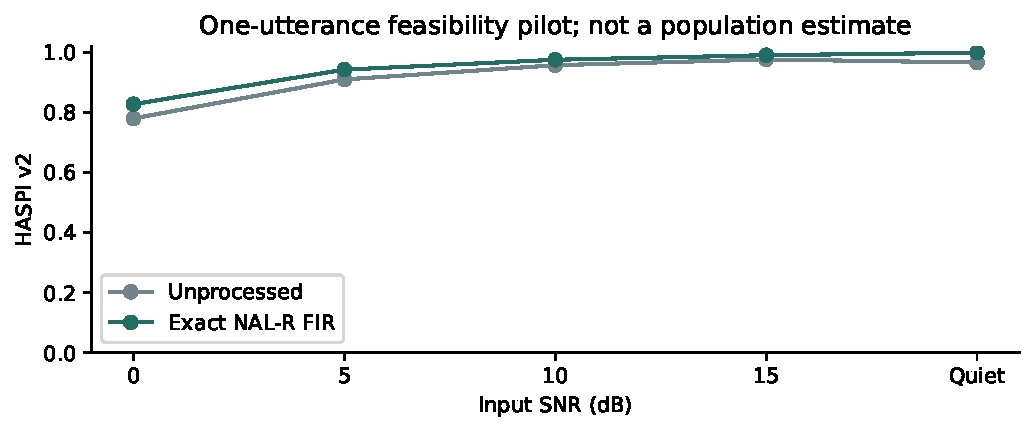
\includegraphics[width=.78\linewidth]{dist/figures/pilot-haspi.pdf}\end{center}
\textbf{Limits on interpretation.} These are five conditions from one utterance, not independent speaker trials. No confidence interval or population conclusion is justified. The quiet and noisy scores need not be monotonically ordered for a nonlinear objective predictor on one short signal. The experiment demonstrates a reproducible evaluator connection and a plausible gain benefit for this case; it does not validate a fitting strategy, neural system or the browser filter bank.

The scoring path retains unbounded floating-point NAL-R output, whose peaks exceed 1.0. Metadata records these peaks. A deployable output ceiling would modify the waveform and must be evaluated separately. Offline MSBG listening files use a shared factor of 0.5 followed by int16 conversion; per-condition loudness normalization is avoided. Acoustic playback calibration remains absent.

\section{Compute measurements and verification}
On AMD EPYC 7763 64-Core Processor with Node v24.22.3, the reconstructed engine measured median 0.179 ms, p95 0.318 ms, p99 0.482 ms and maximum 1.667 ms per block. The measured real-time factor was 0.074; 0 of 3,446 blocks exceeded the 2.902 ms block interval. These are local Node DSP measurements, not browser or hearing-aid hardware measurements.

The benchmark warms the persistent engine for approximately one second and times 3,446 blocks over approximately ten seconds of audio. It includes binaural convolution and the live aid path but excludes audio I/O, browser scheduling, rendering, microphone capture and device conversion. CPU frequency, shared-host load and JIT behavior can change the result. A short run with no observed deadline misses is not a hard real-time guarantee.

Eighteen automated tests cover gain formulas, compressor slope, unity reconstruction, attenuation/delay, output bounds, measured HRIR impulse and ear properties, chunk invariance, worklet telemetry, capture length and sample-rate errors. Syntax and asset/link checks also passed. Browser UI and acoustic-output verification of this reconstructed revision remains pending: browser-control capability was unavailable. Earlier browser checks do not validate this revision.
\newpage
\section{Protocol for a genuine comparative study}
\subsection{Freeze the experiment before choosing a winner}
Use a published hearing-aid benchmark, preferably a specified Clarity task \cite{clarity}, with fixed train/development/test splits. Hold out speakers, rooms and listener profiles where appropriate. Record dataset version, channel ordering, microphone geometry, sample rate, reference definition and dBFS-to-SPL mapping. Include static and moving sources, stationary/dynamic noise, competing speakers, different SNRs and asymmetric losses. Keep every test scene identical across methods.

Compare unprocessed, amplification only, WDRC, enhancement only, and enhancement followed by the same fitting stage. Separate oracle-direction/mask/covariance baselines from estimated versions. Use development data for hyperparameters. Do not optimize an audiogram or select an operating point using test-set scores.

\subsection{Measure a vector of outcomes}
\begin{tabularx}{\linewidth}{@{}p{.24\linewidth}Y@{}}\toprule
Dimension & Required evidence\\\midrule
Intelligibility & Versioned, calibrated HASPI or specified binaural metric; listener testing for benefit claims\\
Quality & HASQI and appropriate quality ratings; do not equate denoising with comfort\\
Spatial preservation & Target/noise ITD and ILD errors; localization under motion and steering error\\
Distortion and output & Peak, clipping rate, spectral/envelope changes and calibrated output constraints\\
Latency and execution & Algorithmic convention, lookahead, frame/hop, group delay, compute tails and loopback delay\\
Embedded feasibility & Peak RAM, parameters, operations, sample format, sustained power/energy\\\bottomrule
\end{tabularx}

HASPI/HASQI incorporate auditory modeling but have validation domains and limitations \cite{haspi}. A normal-hearing quality estimator, SI-SDR or ASR error can be supplementary but cannot replace hearing-aware or listener evaluation. In particular, SI-SDR is insensitive to overall scaling and therefore poorly captures amplification benefit by itself.

Use paired scene-level comparisons, then aggregate with uncertainty at the appropriate speaker/listener unit. Avoid treating many frames from one recording as independent trials. Report failures as well as means. A hearing-impaired listener study requires a suitable protocol and calibrated stimuli; the browser demo is not that study.

\subsection{Implementation milestones}
First add genuine multichannel microphone scenes and causal delay-and-sum/MVDR baselines. Next implement binaural MWF/MWF-N and quantify spatial tradeoffs. Then reproduce one licensed neural checkpoint with persistent streaming state, explicit delay accounting and unchanged downstream fitting. Finally add acoustic feedback, hardware I/O and power measurement. Each module must export its paper, checkpoint hash, configuration, causality, latency and validation status.

\enlargethispage{2\baselineskip}
\textbf{Research conclusion.} Version 0.2 is an executable foundation for asking the right questions and reproducing a small reference experiment. It does not yet establish a state-of-the-art ranking, individual perceptual fidelity or deployable hearing-aid performance.
\newpage
\begin{thebibliography}{99}\small
\bibitem{nidcd} National Institute on Deafness and Other Communication Disorders. \emph{Hearing Aids}; \emph{How Do We Hear?}; \emph{Noise-Induced Hearing Loss}. Official educational resources. \url{https://www.nidcd.nih.gov/health/hearing-aids}; \url{https://www.nidcd.nih.gov/health/how-do-we-hear}. Accessed 25 November 2026.
\bibitem{moore2014} B. C. J. Moore. ``Development and Current Status of the Cambridge Loudness Models.'' \emph{Trends in Hearing}, 2014. \url{https://pmc.ncbi.nlm.nih.gov/articles/PMC4227665/}.
\bibitem{kates2005} J. M. Kates. ``Principles of Digital Dynamic-Range Compression.'' \emph{Trends in Amplification}, 9(2), 45--76, 2005. doi: \href{https://doi.org/10.1177/108471380500900202}{10.1177/108471380500900202}.
\bibitem{moore1997} B. C. J. Moore et al. ``Comparison of real and simulated hearing impairment in subjects with unilateral and bilateral cochlear hearing loss.'' 1997. \url{https://pubmed.ncbi.nlm.nih.gov/9307819/}.
\bibitem{nalr} D. Byrne and H. Dillon. ``The National Acoustic Laboratories' (NAL) new procedure for selecting the gain and frequency response of a hearing aid.'' \emph{Ear and Hearing}, 7(4), 257--265, 1986. doi: \href{https://doi.org/10.1097/00003446-198608000-00007}{10.1097/00003446-198608000-00007}.
\bibitem{mwf} T. Van den Bogaert, S. Doclo, J. Wouters and M. Moonen. ``Speech enhancement with multichannel Wiener filter techniques in multimicrophone binaural hearing aids.'' \emph{JASA}, 125, 360--371, 2009. doi: \href{https://doi.org/10.1121/1.3023069}{10.1121/1.3023069}.
\bibitem{kemar} W. G. Gardner and K. D. Martin. ``HRTF measurements of a KEMAR.'' \emph{JASA}, 97, 3907--3908, 1995. MIT data recorded 1994. \url{https://sound.media.mit.edu/resources/KEMAR.html}.
\bibitem{librispeech} V. Panayotov, G. Chen, D. Povey and S. Khudanpur. ``LibriSpeech: an ASR corpus based on public domain audio books.'' \emph{ICASSP}, 2015. Dataset: \url{https://www.openslr.org/12}, CC BY 4.0.
\bibitem{clarity} Clarity Challenge team. \emph{Clarity software and challenge documentation}. Evaluator implementation: pyclarity 0.9.0. \url{https://github.com/claritychallenge/clarity}; \url{https://claritychallenge.org/clarity_CEC3}. Accessed 25 November 2026.
\bibitem{haspi} J. M. Kates and K. H. Arehart. ``An overview of the HASPI and HASQI metrics for predicting speech intelligibility and speech quality for normal hearing, hearing loss, and hearing aids.'' 2022. \url{https://pubmed.ncbi.nlm.nih.gov/36137862/}.
\bibitem{openmha} \emph{openMHA---An open-source software platform for hearing aid research}. \emph{SoftwareX}, 2022. doi: \href{https://doi.org/10.1016/j.softx.2021.100953}{10.1016/j.softx.2021.100953}.
\bibitem{dfn} H. Schr\"oter, T. Rosenkranz, A. N. Escalante-B. and A. Maier. ``DeepFilterNet: Perceptually Motivated Real-Time Speech Enhancement.'' \emph{Interspeech show and tell}, 2023. \url{https://arxiv.org/abs/2305.08227}.
\bibitem{deepfir} A. Dementyev, C. K. A. Reddy, S. Wisdom, N. Chatlani, J. R. Hershey and R. F. Lyon. ``Towards Sub-millisecond Latency Real-Time Speech Enhancement Models on Hearables.'' 2024; revision 2025. \url{https://arxiv.org/abs/2409.18239}.
\bibitem{wu2025} H. Wu and S. Braun. ``Ultra-Low Latency Speech Enhancement---A Comprehensive Study.'' \emph{ICASSP}, 2025. \url{https://arxiv.org/abs/2409.10358}.
\bibitem{rttango} Z. Benslimane et al. ``RT-Tango: Real-Time Distributed Binaural Speech Enhancement for Low-Power Hearing Aid Devices.'' 2026 preprint. Abstract screened; not reproduced. \url{https://arxiv.org/abs/2607.01834}.
\bibitem{uphaus} L. Uphaus, A. Merboldt, M. Hofbauer and T. Gerkmann. ``Directivity-Conditioned Low-Latency Neural Filtering for Speech Enhancement in Hearing Aids.'' 2026. Abstract screened; not reproduced. \url{https://arxiv.org/abs/2609.15760}.
\end{thebibliography}
\end{document}
